%% -*- coding: utf-8-unix -*-

\chapter{テストシナリオ実装}
\label{chap:poc-scenario-dev}

 \section{テストシナリオの概要}

  \subsection{ネットワークテストの方針}

\ref{chap:poc-target-design}章で設定したとおり、\yo ネットワークのテスト
を考える。そのためのテストシナリオとして「静的なふるまいのテスト」「動的
なふるまいのテスト」の2種類を実装する。テストシナリオ実装・テスト実行を
通して、物理ネットワークのテスト自動実行のポイント検討や問題点の抽出、従
来の人手によるテスト作業との比較を行なう。

  \subsection{BDDテストシナリオの基礎}
  % - TDD/BDDとBDDツールとしてのCucumber
  % - Narrative
  % - ネットワークテストを書く上での検討点、今回のプロジェクトでの方針・決めごと
  %   - なぜそうきめたのか?

      \paragraph{テストツール}
NetTesterはテスト用ノードの生成・テスト対象ネットワークへの配置(パッチ接
続)をおこなうためのAPIを提供する。提供されるAPIを使用して \yo ネットワー
クのテストを実装する。\footnote{実際に作成した自動テストのためのコードは
NetTester Examples~\cite{nettester-ex}として公開している。}

テストシナリオの記述については、アプリケーションのテストでつかわれる既存
のツールと連携することを想定している。本PoCでは、「BDDによるネットワーク
のテスト」を考えていること(\ref{sec:behavior-test}節)、広く使われている
ツールであること、RubyベースでNetTesterとの親和性が高いことをもとに、BDD
ツールであるCucumber\cite{cucumber}を採用した。

    \paragraph{Narrative}
    % Cucumber の .feature の書き方 – NetTester
    %   https://3.basecamp.com/3088280/buckets/867009/messages/155991347
    % クライアントの要望にこたえるWebサービス開発 ~「らせん型ワークフロー」のススメ~
    %  http://www.slideshare.net/mayuco/css-nite-in-sapporo-vol5-14085124
BDDでは、テストのストーリー(フィーチャ)を以下のような構造で記述する
\cite{rspec-book,spiral-workflow}。
\begin{description}
 \item[タイトル] どのストーリーについて説明するのかを示す。タイトルは一
            般に、ユーザがシステムに要求するかもしれないアクティビティを
            短い言葉で表したものになる。
 \item[ナラティブ] ストーリーの内容について説明をする。一般的には
            Connextraフォーマットと呼ばれる形式の短い文章で記述される。
            このテンプレートは、誰がシステムを使っていて、そのユーザは何
            をしていて、なぜそのことに関心があるのか、を明確にする。
            \begin{itemize}
             \item ``As a (role)'': [誰のために(role)]として
             \item ``I want (feature)'': [何を(feature)]したい
             \item ``So that (bussiness value)'': なぜなら[なぜ
                   (bussiness value)]のためだ
            \end{itemize}
 \item[受け入れ基準] ストーリーの完了・完成を定義する受け入れ基準、シナ
            リオの定義。
\end{description}

Cucumberにおけるフィーチャとは、システムを利用するユーザーまたは別のコン
ピュータの視点に立っておおまかに表現された要件のことを指す。Cucumberの
フィーチャはタイトルと簡単なナラティブ、受け入れ基準としての役割をはたす
自動化されたシナリオによって構成される。
\begin{itemize}
 \item フィーチャはタイトルとナラティブで構成され複数のシナリオを含む。
       (本プロジェクトでは\verb|features/*.feature|ファイル)
       \begin{itemize}
        \item シナリオはそれぞれ、シナリオ内でおこることを任意のステップ
              で記述する。
       \end{itemize}
 \item 個々のステップ定義は開発で使っているシステムの言語で記述される。
       (本プロジェクトではRuby: \verb|features/step_definitions/*.rb|ファ
       イル)
\end{itemize}

% Narrative を Pull Requst する – NetTester
%   https://3.basecamp.com/3088280/buckets/867009/todos/159223633
% NetTester機能拡張(NW機器間接続)方針・やりたいこと – NetTester
%   https://3.basecamp.com/3088280/buckets/867009/todos/182746431
% Firewall の cucumber シナリオ – NetTester
%   https://3.basecamp.com/3088280/buckets/867009/todos/158299550

 \section{静的なふるまいのテストの実装}
% テストシナリオ策定の考えかた…そもそもなにをするテストなのか。どのような
% 検討を経てテストシナリオをきめたのか。narrativeの定義のプロセスとか。
% TODO: OOD資料にかいたようなテストコード解説のはなしをこちらにも含めるか?
% - 実装
%   - Step2テスト業務で気づいたことをまとめる – NetTester
%     \url{https://3.basecamp.com/3088280/buckets/867009/todos/260220903}

  \subsection{テストとして実現したいこと}
ネットワークに対して最低限要求されることは、ネットワークを介して必要な通
信が実現できることである。ネットワークの目的は、大きく言えばコミュニケー
ションを実現することである。あるノードが、他のノードと、必要な手段(アプ
リケーション)で通信できるかどうか、という点がまず初めにネットワークに求
められる機能要求となる。

「ネットワークの静的なふるまい」(\ref{sec:behavior-to-test}参照)では、ネッ
トワークが定常状態にある(一定の状態にあって状態変化しない)ときに、ネット
ワーク利用者が実現したいend-to-endの通信がすべて実現可能かどうかをテスト
する。

  \subsection{テスターに求められる機能}

テストで確認したいend-to-endの通信、すなわち、実現したい通信要求は、通信
をおこなうノード(エンドポイント)の論理的・物理的な配置の組合せに応じて異
なる。また、通信をおこなうアプリケーションによっても別途制御がおこなわれ
る。例えば、LBやDPI\footnote{Deep Packet Inspection}をおこなうFWなどがネッ
トワーク内にある場合は、単純な宛先(ヘッダ)情報だけではなく、やりとりされ
るアプリケーションレベルの情報によって通信の可否などが変化する。

したがって、単純なend-to-endの通信試験だとしても、配置やアプリケーション
の組合せによって大量のテストケースが発生してしまう、テストのためのリソー
ス確保などが充分にできない、などの課題があった
(\ref{sec:discuss-network-test}参照)。

そこで、テスター(NetTester)では以下の機能が要求される。
\begin{itemize}
 \item テスト用ノードの生成
 \item テスト用ノードの配置
 \item テスト用ノード上でのタスク実行
 \item 複数のテスト用ノード操作/集中管理
\end{itemize}
NetTesterはこうしたノードの生成・配置・集中制御の機能(API)を提供している。
テストシナリオ(Cucumber)ではBDDの考えかたに基づいて、ノード間でどういっ
た通信を実現する必要があるかを個別の通信要件
(\tabref{tab:poc-requires-yo-int},\tabref{tab:poc-requires-yo-dmz},\tabref{tab:poc-requires-etc})
ごとに定義する。

 \section{動的なふるまいのテストの実装}
% 障害試験シナリオを書く – NetTester
% \url{https://3.basecamp.com/3088280/buckets/867009/todos/238169066}
% Step2to3タスク検討
% https://drive.google.com/open?id=0B2eRR_JxYJA5M1RGdEZaOFkxTFk

  \subsection{テストとして実現したいこと}
% NetTester機能拡張検討
% https://drive.google.com/file/d/0B2eRR_JxYJA5TmhaeWItNF93Um8/view
ネットワークは状況に応じて状態を変化させる。変化のトリガとして、例えば障
害発生による冗長経路への切替、メンテナンスのための一部のデバイスの停止や
切り離し・そのための通信経路迂回、ネットワーク機器の追加(拡張)や削除(縮
小)などがある。こうしたイベントに対して、ネットワーク(全体)は、ネットワー
クの状態と発生したイベントに応じて自らの情報(状態)を自律的に更新し、トラ
フィックの経路を変更するなどの制御をおこなう。

「ネットワークの動的なふるまい」(\ref{sec:behavior-to-test}参照)では、ネッ
トワークが状態変化するときに、ネットワーク利用者へ与える影響が許容範囲内
かどうかをテストする。ネットワーク利用者への影響とは、ネットワーク状態遷
移中に発生するトラフィックの継続可否、影響度・影響範囲(場所的な範囲や時
間)である。例を以下にあげる。
\begin{itemize}
 \item トラフィックの継続可否
       \begin{itemize}
        \item ロードバランサなどL7の情報にしたがってトラフィックを操作す
              るような機器では、冗長系切替のときに、セッション情報などを
              引きついでアプリケーション通信を維持することが求められる。
              同様にNATなどの変換テーブルに基づいてトラフィックを操作す
              る機器でも冗長系機器間で状態の同期が必要になる。
        \item 系切替には隣接する機器も関連する。例えば、対象とする冗長系
              のL1/L2の切替に Gratuitous ARP を使用する機器で、隣接する
              L2スイッチのバグによって Gratuitous ARP 処理が正しくおこな
              われず、全体としてトラフィックの継続に失敗した事例などがあ
              る。
       \end{itemize}
 \item 影響度・影響範囲
       \begin{itemize}
        \item 状態変化によって予期しない現象が予期しない範囲でおこること
              がある。範囲としては、物理的な場所(特定のスイッチの配下な
              ど)・論理的な場所(特定のL2セグメントなど)複数の要素が考え
              られる。
        \item 仮想化によって物理構成と論理構成は分離されることが一般的で
              ある。この際、物理構成操作のオペミスや論理構成操作のミス
              (記述ミスや勘違い)によったわずかなミスの見落としがセグメン
              ト全体をまきこむL2ループを引き起すことがある。
        \item 機器のバグや設定ミス、そのほかの機能との併用による機器CPU
              専有状況の発生などがあると、こうした系切替によるトラフィッ
              クの維持・継続ができなかったり、想定した時間内に完了できな
              いことがある。例として、多数のVLANを収容していたL3スイッチ
              で、系切替の際のSTPトポロジ再計算処理によるCPU専有が発生し、
              スイッチ配下のセグメント全域で広範囲にわたって切替時間の遅
              延・それにともなうトラフィックの維持失敗(タイムアウト発生)
              がおこってしまった事例などがある。
       \end{itemize}
\end{itemize}

いくつか例を挙げたが、これらの問題はネットワーク全体(系全体)の相互作用に
影響される。ネットワークの場合はベンダや機器ごとに独自のOSやアーキテクチャ
を持つものが多く、特定機能や製品を組み合わせたときの相性問題やキャパシティ
問題、特定ハードウェアやソフトウェア(バージョン)のトラブルといった情報を
共有することは難しい。また、複数の冗長化機能(複数の機器にまたがるものも
含む)の連動する際、状態遷移のタイミングなどで機能単体では問題なく動作す
る機能が複合した結果、問題が発生することもある\footnote{例として:
OSPF/BGP収束時間差によるブラックホールやループの発生
\cite{j3g14-packet-forwarding}など。}。こうした理由により、ネットワーク
の操作・状態変化において、すべての影響を予想するのは非常に困難である。

動的なふるまいのテストでは、上に挙げた「トラフィックの継続可否」「影響度・
影響範囲」のテストを自動化することを目標とする。

  \subsection{テスターに求められる機能}
  % 求められる機能、今回実装したもの

「動的なふるまいのテスト」では、次のような機能が必要となる。
\begin{description}
 \item[イベントの生成] ネットワークの状態変化を発生させるためのイベント
            を発生させる機能。今回のPoCではリンク障害試験をターゲットと
            するので、何らかの形でリンク障害を発生させる必要がある。
 \item[イベント発生時のトラフィック影響調査] ネットワークが状態変化する
            タイミングで、ネットワーク上のトラフィックがどの程度の影響を
            うけているかを調査する必要がある。
\end{description}

一般的には、ネットワークの状態変化イベントによって影響をうけることが予想
されるトラフィックをあらかじめ生成しておき、イベント発生・ネットワーク状
態変化の収束をまって、トラフィックに最終的にどのような影響があったのかを
調査する。したがって、複数のノード間において・同時並行で・トラフィックを
継続生成(送受信)しながらイベントを発生させる機能が必要となる。

  \subsection{システム構成}
PoC環境(詳細は\figref{fig:poc-env-physical-detail})では
\figref{fig:poc-env-linkdown}のようにtester set 1を「動的なふるまいのテ
スト」用に使用するよう設計している。PoCでは、\yo 内部ネットワークの中心
となるFWの冗長化機能試験をおこなう。そのため、テストシナリオではFWの
Active/Passive切替トリガとなるActive側(FW1)リンクダウン/リンクアップ操作
を実装する。物理リンク操作のため物理OpenFlowスイッチ(OFS1)へ以下の2リン
クをそれぞれ引き込んでいる。
\begin{itemize}
 \item L3SW-FW1 間リンク (FW1 Uplink)
 \item FW1-L2SW1 間リンク (FW1 Downlink)
\end{itemize}

\begin{figure}[h]
 \centering
 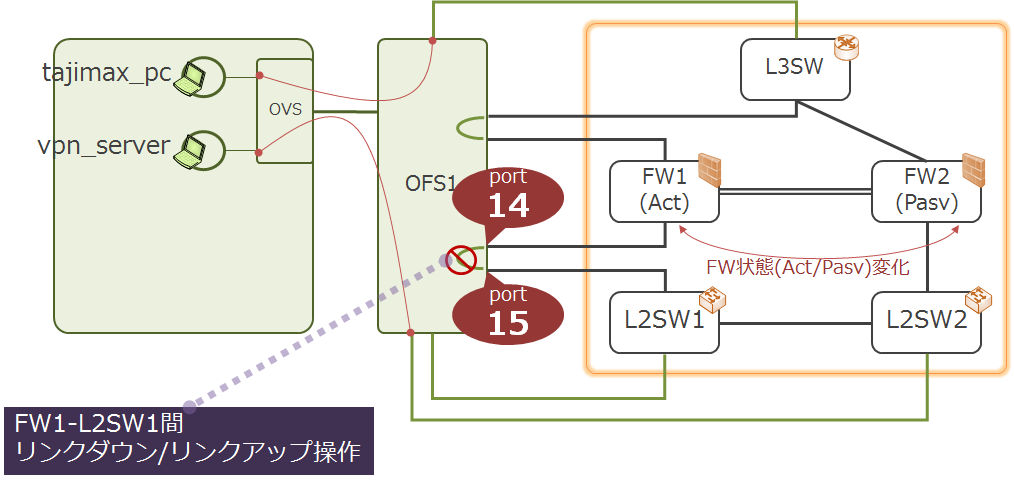
\includegraphics[scale=0.6]{img/poc-env-linkdown.png}
 \caption{PoC環境: NetTesterによるリンクダウン操作}
 \label{fig:poc-env-linkdown}
\end{figure}

 \section{テストシナリオ実装における検討ポイント}

  \subsection{Teardown処理}

CI/CDといったプロセスを実現する上で、複数・任意のテストシナリオをまとめ
て実行することが求められる(回帰テスト含む)。

テストシナリオはいずれも、テスト対象が所定の初期状態にあるところから実行
を開始しなければ狙った「ふるまい」を調査することができない。ソフトウェア
の自動テストでは、テスト対象となるアプリケーション(プロセス)やインスタン
スは初期状態で起動しなおすことが容易なため、常にアプリケーションやインス
タンスを起動しなおして初期状態からのテストをおこなうのが一般的である。

しかし、ネットワーク(特に物理ネットワーク)を対象としている場合はテスト対
象が物理的に存在している。よって、そのままでは、前のテストシナリオ実行直
後のネットワーク状態が次のテストシナリオ実行開始時の初期状態となってしま
う。個々のテストシナリオ実行のたびにネットワーク(機器)の初期化・再構築す
ることは、不可能ではないが以下の理由により難しい。
\begin{itemize}
 \item 機器によっては、コンフィグ消去・再起動に数分から十数分かかるもの
       がある。
 \item 再起動によるteardown処理をおこなう場合、ネットワーク機器の起動順
       序によりネットワーク全体の状態が変化し得る。
 \item コンフィグリセット操作に失敗すると再起動後にリモートアクセスでき
       ず、復旧作業(現地作業)が必要になるリスクがある。
\end{itemize}
特に本PoCでは、静的なふるまいのテストとして数十の通信要件をテストするた
めのシナリオを連続実行したいという要求があるため、単一テストシナリオ実行
の時間的なオーバーヘッドが大きいことが問題となる。

そのため、テストに応じて何らかの形でネットワークの状態を初期状態に戻すた
めの処理(teardown処理)を実装する必要がある。本PoCではL2-L4の状態に着目し
て、以下のteardown操作を実装している。

    \paragraph{Target network の状態操作}
テスト対象ネットワーク各機器のL2-L4の状態をクリアする(CLIによる各種
\code{clear}コマンドの実行)。
\begin{itemize}
 \item MACアドレステーブル/ARPキャッシュのクリア
 \item FWの NAT Table のクリア
 \item FWの active/standby 状態のクリア
       \begin{itemize}
        \item 今回、動的なふるまいのテストにあたって、FWは障害が発生した
              リンクの復旧にあわせて active/passive を自動復旧するように
              設計したため、特に操作していない
              (\ref{sec:physical_nw_design}参照)。
       \end{itemize}
\end{itemize}

    \paragraph{Netns の /etc 配下のSetup/Teardown}
    % 自作echoサーバーで通信開始時に10秒のラグが起きる問題 – NetTester
    % https://3.basecamp.com/3088280/buckets/867009/todos/274457003

NetTesterでは、Network namespace でテスト用ホストを生成する。このときバッ
クエンドでは iproute2(\code{ip}コマンド)を使用している。iproute2 によっ
て生成されたホスト(netns)では、\verb|/etc/netns/<netns>/| が etc ディレ
クトリとしてマウントされる~\cite{iproute2-doc}。そのため、テスト用ホスト
内部での名前解決などでは、実体としては \verb|/etc/netns/<netns>/hosts|,
\verb|resolv.conf| を参照する。これらの設定ファイル等が正しく設定されて
いないと名前解決がタイムアウトするなどの問題が発生する。

    \paragraph{物理OFSのflow tableのクリア}
物理OpenFlowスイッチには、テストのたびにフローエントリが登録される。その
ため、テストの実行のたびにフローエントリのクリア処理が必要となる。

本PoCでは、テスト用ホストのMACはテスト実行時にランダムに設定するよう実装
したため、テスト実行をくりかえすと多数の不要なフローエントリが物理スイッ
チ上に残る。テスト用ホストのMACアドレスを固定にすることでフローテーブル
の消費は抑えられるが、異なる用途で同一のMACアドレスを使いまわすなどのケー
スで、予期しない動作不具合が発生するおそれがある\footnote{NetTesterのテー
ブル設計では、テスト用ホストのMACアドレスをキーとして、フロー優先度
(priority)による制御をおこなう(\ref{sec:flow-priority-design}参照)。同一
MACアドレスを異なる用途で使いまわす場合、他の用途として設定したフローエ
ントリとマッチしてしまい、狙ったパッチ動作が実現できない恐れがある。}点
に注意すること。

\section{並列実行と排他制御}

物理ネットワークをテストする場合、テスト対象(物理ネットワーク)は原則ひと
つしかない。テストの数が多くなる場合、複数のテストを同時に実行することが
考えられるが、現状NetTesterを使ったテスト自動化は並行実行は原則としてで
きない。以下にその理由を列挙する。

\begin{description}
 \item[状態操作の競合] テストシナリオごとに、想定しているテスト対象ネッ
            トワークの状態がある。それらを変化させるテストシナリオは同時
            に実行できない。
            \begin{itemize}
             \item テストシナリオAを実行している途中で、テストシナリオB
                   がteardown処理を実行して、テスト対象ネットワークの状
                   態クリアをしてしまうと、テストシナリオAで想定していた
                   状態を変化させてしまう\footnote{Teardown処理として
                   \code{clear}コマンドを使用しているが、特定シナリオで
                   使うエントリだけを消去するのではなく、NW機器全体の情
                   報をまとめて消去してしまうため。そのシナリオに依存す
                   るエントリだけをねらって消去できるのであればこの制約
                   は外れるが、テスト対象ネットワーク内の機器それぞれに
                   ついて対応可能かどうかという点が問題となるだろ
                   う。}\footnote{あるいは、teardown処理を他のテストシナ
                   リオ実行がおわるまで待機し、まとめて実行できればよい
                   が、現状はそうした実装をおこなっていない。}。
             \item 動的なふるまいのテストのように、ネットワーク全体の状
                   態に影響をあたえるようなテストシナリオは同時に実行で
                   きない。
            \end{itemize}
 \item[ネットワークリソースの競合] テスト対象ネットワークで一意でなけれ
            ばならないリソースの操作については同時に実行できない。
            \begin{itemize}
             \item テストシナリオA/Bが同じIP/MACを持つテスト用ホストを同
                   時に生成してしまうと、テスト対象ネットワーク内で
                   IP/MACの重複が発生してしまう。
             \item 物理リンクの操作など、ひとつしか存在しないリソースの
                   制御が必要なテストシナリオは同時に実行できない。
            \end{itemize}
\end{description}

本PoCでは\figref{fig:poc-env-physical-detail}のようにふたつのtester set
を使用しているが、これはあくまでもデバッグ用途のためである。Tester set
を複数用意することで、静的なふるまいのテスト(NWが定常状態にある)で、かつ
同じIP/MACのテスト用ノードを使用せず、teardown 処理をテストシナリオ単位
で実行しないようなケースに限って複数のテストが実行可能となる。

上記の制約の一部については、NetTesterで実行されるタスクの排他制御のしく
みを導入することで対応できるものがあるが、現状はそうした対応については本
PoCの範囲外としている。本PoCでは、ひとつのテスト対象ネットワークに対して
tester setがあり、同時にひとつのテストシナリオを実行することが前提となっ
ている。

\subsection{テストシナリオのサイズ}

シナリオサイズの目安、シナリオ分割の目安 (step3 test つくっているときに
分割するって話になった理由は?)

\subsection{ステップ実装上の工夫}
\begin{itemize}
 \item ニセ○○サーバとステップ実装 – NetTester \url{https://3.basecamp.com/3088280/buckets/867009/documents/216490375}
 \item コマンドをバックグラウンド実行 – NetTester \url{https://3.basecamp.com/3088280/buckets/867009/documents/216399643}
 \item step内でのバックグラウンドコマンド実行 – NetTester \url{https://3.basecamp.com/3088280/buckets/867009/todos/202691188}
 \item factory\_girl で仮想ホストを作る – NetTester \url{https://3.basecamp.com/3088280/buckets/867009/documents/210831650}
\end{itemize}

\section{PoCの結果と評価}

\subsection{実際に発見できた問題点}
テストとしての結果まとめ
\begin{itemize}
  \item 結果: 実際に発見できたトラブルや設定ミスなどをあげる。
       \begin{itemize}
        \item Teardown関連
              \begin{itemize}
               \item 原因切り分けメモ (muraki) – NetTester \url{https://3.basecamp.com/3088280/buckets/867009/documents/217782147}
               \item 調査: テスト環境でシナリオ実行すると2回目以降でコケる – NetTester \url{https://3.basecamp.com/3088280/buckets/867009/todos/218486066}
              \end{itemize}
        \item Target Network の設定不備の発見
              \begin{itemize}
               \item DNSのテスト作る – NetTester \url{https://3.basecamp.com/3088280/buckets/867009/todos/301325453}
               \item 通信要件\#10 A社内PC→インターネットの疎通確認(ICMP) – NetTester \url{https://3.basecamp.com/3088280/buckets/867009/todos/233175867}
               \item 通信要件\#29 B社PC→DMZ内のVPNサーバの疎通確認(SSLVPN) – NetTester \url{https://3.basecamp.com/3088280/buckets/867009/todos/233178490}
              \end{itemize}
       \end{itemize}
\end{itemize}

step3
\begin{itemize}
 \item 実装 (NAT IPの変更とかデモの話をどこまで含めるか?)
 \item 結果
\end{itemize}

\subsection{ネットワークの構築・運用プロセスに対する定性的な評価}
評価・考察
\begin{itemize}
 \item 体制や役割分担/タスクとスキルセットについて: ref.\url{https://3.basecamp.com/3088280/buckets/867009/todos/260220903}
 \item テスト実装のコスト
 \item 繰り返し実行できることのメリット
       \begin{itemize}
        \item OSの更新などおおきな変更にたいするリスクヘッジ
       \end{itemize}
\end{itemize}


%%% Local Variables:
%%% mode: yatex
%%% TeX-master: "main.tex"
%%% End:
